% ===================================================================================== %
%                                        Header                                         %
% ===================================================================================== %
\documentclass[10pt,t,xcolor=table,compress]{UWMadBeamer}

\usepackage{graphicx}
\usepackage{transparent}
\usepackage{textcomp}
\usepackage{lmodern}
\usepackage{amsmath}
\usepackage{setspace}
\usepackage{booktabs}
\usepackage{multirow}
\usepackage{appendixnumberbeamer}



% =============================================================================================== %
%                                     Math Commands                                               %
% =============================================================================================== %


% ---------------------------------------------------------------------------- %
%                                Square Root Tail                              %
% ---------------------------------------------------------------------------- %
\DeclareRobustCommand{\NthRootInTeX}[2]{\root #1 \of {#2\:\!}}

\DeclareRobustCommand{\SquareRootCore}[2]{
    \setbox0=\hbox{\ensuremath{\NthRootInTeX{#1}{#2}}}
    \dimen0=\ht0
    \advance\dimen0-0.2\ht0
    \setbox2=\hbox{\vrule height\ht0 depth -\dimen0}
    {\box0\lower0.47pt\box2}
}

\DeclareRobustCommand{\Sqrt}[2][]{
    \mathchoice{\SquareRootCore{#1}{#2}}
               {\SquareRootCore{#1}{#2}}
               {\SquareRootCore{#1}{#2}}
               {\SquareRootCore{#1}{#2}}
}



% ---------------------------------------------------------------------------- %
%                              Derivative Commands                             %
% ---------------------------------------------------------------------------- %
\newcommand{\bigdiffn}[4]{\dfrac{#1{}^{#4}}{#1 #3{}^{#4}} \left[ #2 \right]}
\newcommand{\gendiffn}[4]{\dfrac{#1{}^{#4} #2}{#1 #3{}^{#4}}}

\newcommand{\diff}[3][d]{
    \ifthenelse{\equal{p}{#1}}{
        \gendiffn{\partial}{#2}{#3}{}
    }{
        \ifthenelse{\equal{b}{#1}}{
            \bigdiffn{d}{#2}{#3}{}
        }{
            \ifthenelse{\equal{bp}{#1}}{
                \bigdiffn{\partial}{#2}{#3}{}
            }{
                \gendiffn{d}{#2}{#3}{}
            }
        }
    }
}

\newcommand{\diffn}[4][d]{
    \ifthenelse{\equal{p}{#1}}{
        \gendiffn{\partial}{#2}{#3}{#4}
    }{
        \ifthenelse{\equal{b}{#1}}{
            \bigdiffn{#2}{#3}{#4}
        }{
            \ifthenelse{\equal{bp}{#1}}{
                \bigdiffn{\partial}{#2}{#3}{#4}
            }{
                \gendiffn{#1}{#2}{#3}{#4}
            }
        }
    }
}

\newcommand{\bigdiff}   [2] {\diff[b]{#1}{#2}}
\newcommand{\pdiff}     [2] {\diff[p]{#1}{#2}}
\newcommand{\bigpdiff}  [2] {\diff[bp]{#1}{#2}}
\let\frac\dfrac
\newcommand{\subs}      [2][]{\ensuremath{{}_{#1\text{\scriptsize #2}}}}
\newcommand{\sups}      [2][]{\ensuremath{{}^{#1\text{\scriptsize #2}}}}
\newcommand{\oneo}      [1]  {\ensuremath{\frac{1}{#1}}}




\newcommand{\Density}{\ensuremath{\rho}\xspace}
\newcommand{\Temperature}{\ensuremath{T}\xspace}
\newcommand{\Pressure}{\ensuremath{P}\xspace}
\newcommand{\IntEnergy}{\ensuremath{i}\xspace}
\newcommand{\Entropy}{\ensuremath{s}\xspace}
\newcommand{\Enthalpy}{\ensuremath{h}\xspace}
\newcommand{\ThCond}{\kappa}
\newcommand{\Viscosity}{\mu}
\newcommand{\DiffCoef}{\ensuremath{D}\xspace}

\newcommand{\isat}{\ensuremath{\IntEnergy\subs[\!]{sat}}\xspace}
\newcommand{\Psat}{\ensuremath{\Pressure\subs[\!\!]{sat}}\xspace}
\newcommand{\Tsat}{\ensuremath{\Temperature\subs[\!\!\:]{sat}}\xspace}
\newcommand{\SubL}{\subs[\!\!\:]{\rule{0pt}{8pt}$\textstyle\ell$}}
\newcommand{\SubG}{\subs[\!\!\:]{$\mathit{g}$}}

\newcommand{\rhol}{\ensuremath{\rho\SubL}\xspace}
\newcommand{\rhog}{\ensuremath{\rho\SubG}\xspace}
\newcommand{\il}{\ensuremath{i\SubL}\xspace}
\newcommand{\ig}{\ensuremath{i\SubG}\xspace}
\newcommand{\rhoul}{\ensuremath{\rhou\SubL}\xspace}
\newcommand{\rhoug}{\ensuremath{\rhou\SubG}\xspace}
\newcommand{\rhoil}{\ensuremath{\rhoi\SubL}\xspace}
\newcommand{\rhoig}{\ensuremath{\rhoi\SubG}\xspace}
\newcommand{\alphal}{\ensuremath{\alpha\SubL}\xspace}
\newcommand{\alphag}{\ensuremath{\alpha\SubG}\xspace}

\newcommand{\tauSat}{\ensuremath{\tau\subs[\!\!\:]{sat}}\xspace}
\newcommand{\deltaL}{\ensuremath{\delta\subs[\!\!\:]{\rule{0pt}{8pt}$\textstyle\ell$}}\xspace}
\newcommand{\deltaG}{\ensuremath{\delta\subs[\!\!\:]{$\mathit{g}$}}\xspace}

\newcommand{\rhoc}  {\ensuremath{\rho\subs{c}}\xspace}
\newcommand{\Tc}    {\ensuremath{T\subs{c}}\xspace}

\newcommand{\Skip}[1][0.45em]{\\[#1]}
\newcommand{\TCS}    {Thermodynamic Coexistence System\xspace}
\newcommand{\TCSRef} {\hyperref[Eqn:TCS]{\TCS}\xspace}
\newcommand{\MCS}    {Mechanical Coexistence System\xspace}
\newcommand{\MCSRef} {\hyperref[Eqn:MCS]{\MCS}\xspace}

\newcommand{\Afe}{\ensuremath{A\subs{\textsc{fe}}}}
\newcommand{\HFE}{Helmholtz free energy\xspace}
\newcommand{\EOS}{equation of state\xspace}

\newcommand{\Space}{\ensuremath{z}\xspace}
\newcommand{\Time}{\ensuremath{t}\xspace}
\newcommand{\Speeds}{\ensuremath{\mathbf{\lambda}}\xspace}

\DeclareMathOperator{\Ln}{Ln}
\DeclareMathOperator{\Abs}{Abs}
\DeclareMathOperator{\Inf}{Inf}
\DeclareMathOperator{\Exp}{Exp}
\DeclareMathOperator{\Rez}{R}

\let\originalleft\left
\let\originalright\right
\renewcommand{\left}{\mathopen{}\mathclose\bgroup\originalleft\;\!}
\def\left#1{\mathopen{}\mathclose\bgroup\originalleft#1\:\!}
\def\right#1{\aftergroup\egroup\:\!\originalright#1}


%\DefineNewLength{\RowSkip}{1.0em}
%\newcommand{\skp}[1][0.45em]{
%    \ifthenelse{\equal{#1}{}}{
%        \\[\RowSkip]
%    }{
%        \\[#1]
%    }
%}

\newcommand{\Del}[1][]{
    \partial_{#1}
}

\newcommand{\Vector}[1]{
    \underline{#1}
}

\newcommand{\Tensor}[1]{
    \underline{\underline{#1}}
}

\newcommand{\qConRaw}{\mathbf{q}}
\newcommand{\qCon}{\ensuremath{\qConRaw}\xspace}
\newcommand{\qPer}{\ensuremath{\widehat{\qConRaw}}\xspace}
\newcommand{\qSS} {\ensuremath{\qConRaw^0}\xspace}

\newcommand{\ConSys}{
    \Psi
}

\newcommand{\ConSysHEM}[1][HEM]{
    \ConSys_{\!\mbox{\tiny #1}}
}


\newcommand{\Flux}{
    \mathbf{F}
}
\newcommand{\Source}{
    \mathbf{S}
}

\newcommand{\Weight}{\beta}


\newcommand{\FluxFun}[2][]{
    \mathbf{F}_{#1}\left(#2\right)
}

\newcommand{\SourceFun}[2][]{
    \mathbf{S}_{#1}\left(#2\right)
}

\newcommand{\ResidualFun}[2][]{
    \mathbf{R}_{#1}\left(#2\right)
}

\newcommand{\Jacobian}[1][]{
    \mathbb{J}\subs{#1}
}

\newcommand{\JacobGen}[2]{
  \Jacobian[{\scriptscriptstyle #1}](#2)
}

\newcommand{\JacobF}{
    \Jacobian[F]
}


\newcommand{\JacobS}[1]{
    \JacobGen{S}{#1}
}

\newcommand{\FluxSS}{
    \mathbf{F}^{0}
}

\newcommand{\SourceSS}{
    \mathbf{S}^{0}
}

\newcommand{\JacobFSS}[1][\,\,\!]{
    \mathbf{J}_{\!{\scriptscriptstyle F}}^{0}{}#1
}

\newcommand{\JacobSSS}[1][\,\,\!]{
    \mathbf{J}_{\!{\scriptscriptstyle S}}^{0}#1
}

\newcommand{\BigO}[1]{
    \ensuremath{\mathcal{O}\!\left(#1\right)}
}


\newcommand{\Correl}[2]{
    f^{\mbox{\scriptsize cor}}_{#1}\left(#2\right)
}

\newcommand{\LpNorm}[2][2]{
    \ensuremath{\lvert\!\lvert#2\rvert\!\rvert_{#1}}
}

\newcommand{\Nudge}{
    \ensuremath{\!\!\;}
}

\newcommand{\hfg}{
    \ensuremath{h_{\mbox{\scriptsize fg}}}
}



%\NewEnviron{BoxedAlgorithm}[1][H]{
%    \begin{center}
%        \begin{minipage}{0.999\textwidth}
%            \centering
%            \fcolorbox{black}{white}{
%                \centering
%                \begin{minipage}[t]{0.85\textwidth}
%                    \begin{algorithm}[#1]
%                        \BODY
%                    \end{algorithm}
%                \end{minipage}
%            }
%        \end{minipage}
%    \end{center}
%}


\DeclareRobustCommand{\TH}  {thermal hydraulics\xspace}
\DeclareRobustCommand{\THc} {Thermal hydraulics\xspace}
\DeclareRobustCommand{\THcc}{Thermal Hydraulics\xspace}
\DeclareRobustCommand{\THs} {thermal hydraulic\xspace}

\DeclareRobustCommand{\CLaw}  {conservation law\xspace}
\DeclareRobustCommand{\CLaws} {conservation laws\xspace}


\newcommand{\rhou}{\ensuremath{\rho{u}}\xspace}
\newcommand{\rhoi}{\ensuremath{\rho{i}}\xspace}

\newcommand{\tr}{\ensuremath{{}\sups{\textsc{T}}}}
\newcommand{\mdotloss}[1][]{\ensuremath{\dot{m}'''\subs[\!\!\!\!\!#1]{loss}}\xspace}
\newcommand{\Keff}{\ensuremath{K\subs{eff}}}

\newcommand{\POfRhoRhoi}{\ensuremath{P\left(\rho,\frac{\rhoi}{\rho}\right)}}


\newcommand{\EqnSkip}[1][3em]{\ensuremath{\mbox{\rule{0.5em}{#1}}}\\}
\newcommand{\psiEOS}{\ensuremath{\psi}\subs{\textsc{eos}}}




%\DefineNewLength{\BarredLetterHeight}{0pt}
%\DefineNewLength{\BarredLetterWidth}{0pt}

%\newcommand{\eBB}{
%    \ensuremath{
%        \settoheight{\BarredLetterHeight}{e} % Height in current context
%        \settowidth{\BarredLetterWidth}{e}   % Width  in current context
%        e\mbox{\hspace{-0.57\BarredLetterWidth}\rule{0.035em}{0.96\BarredLetterHeight}} % bar
%    }
%}

%\newcommand{\TableSkip}{\rule[-1.4em]{0pt}{3.3em} \\[0pt]}
\definecolor{Gray}{gray}{0.93}


\newcommand{\LedineggCriterion}{$\tfrac{\partial\Delta{P}}{\partial(\rhou)}\bigr\rvert_{\text{int}} \le 
                                 \tfrac{\partial\Delta{P}}{\partial(\rhou)}\bigr\rvert_{\text{ext}}$}
                                
                                
\newcommand{\etal}{et al.\xspace}
\newcommand{\etc}{etc.\xspace}
\newcommand{\eg}{e.g.\xspace}
\newcommand{\ie}{i.e.\xspace}


\newcommand{\rhok}{ \ensuremath{\alpha\rho\subs{\phi}}\xspace}
\newcommand{\rhouk} {\ensuremath{\alpha\rhou\subs{\phi}}\xspace}
\newcommand{\rhoik} {\ensuremath{\alpha\rhoi\subs{\phi}}\xspace}
\newcommand{\alphak}{\ensuremath{\alpha\subs{\phi}\xspace}}
\newcommand{\uk}{\ensuremath{u\subs{\phi}}\xspace}
\newcommand{\ik}{\ensuremath{i\subs{\phi}}\xspace}
\newcommand{\CVvol}[1][k]{\ensuremath{\Omega_\text{#1}}\xspace}
\newcommand{\MCvol}[1][m]{\ensuremath{\Omega_\text{#1}}\xspace}
\newcommand{\CVsurf}[1][k]{\ensuremath{\Gamma_\text{#1}}\xspace}
\newcommand{\MCsurf}[1][m]{\ensuremath{\Gamma_\text{#1}}\xspace}








    \let\Oldalpha     \alpha     \renewcommand{\alpha}     {\ensuremath{\Oldalpha     }\xspace}
    \let\Oldbeta      \beta      \renewcommand{\beta}      {\ensuremath{\Oldbeta      }\xspace}
    \let\Oldgamma     \gamma     \renewcommand{\gamma}     {\ensuremath{\Oldgamma     }\xspace}
    \let\Olddelta     \delta     \renewcommand{\delta}     {\ensuremath{\Olddelta     }\xspace}
    \let\Oldepsilon   \epsilon   \renewcommand{\epsilon}   {\ensuremath{\Oldepsilon   }\xspace}
    \let\Oldvarepsilon\varepsilon\renewcommand{\varepsilon}{\ensuremath{\Oldvarepsilon}\xspace}
    \let\Oldzeta      \zeta      \renewcommand{\zeta}      {\ensuremath{\Oldzeta      }\xspace}
    \let\Oldeta       \eta       \renewcommand{\eta}       {\ensuremath{\Oldeta       }\xspace}
    \let\Oldtheta     \theta     \renewcommand{\theta}     {\ensuremath{\Oldtheta     }\xspace}
    \let\Oldvartheta  \vartheta  \renewcommand{\vartheta}  {\ensuremath{\Oldvartheta  }\xspace}
    \let\Oldkappa     \kappa     \renewcommand{\kappa}     {\ensuremath{\Oldkappa     }\xspace}
    \let\Oldlambda    \lambda    \renewcommand{\lambda}    {\ensuremath{\Oldlambda    }\xspace}
    \let\Oldmu        \mu        \renewcommand{\mu}        {\ensuremath{\Oldmu        }\xspace}
    \let\Oldnu        \nu        \renewcommand{\nu}        {\ensuremath{\Oldnu        }\xspace}
    \let\Oldxi        \xi        \renewcommand{\xi}        {\ensuremath{\Oldxi        }\xspace}
    \let\Oldpi        \pi        \renewcommand{\pi}        {\ensuremath{\Oldpi        }\xspace}
    \let\Oldvarpi     \varpi     \renewcommand{\varpi}     {\ensuremath{\Oldvarpi     }\xspace}
    \let\Oldrho       \rho       \renewcommand{\rho}       {\ensuremath{\Oldrho       }\xspace}
    \let\Oldvarrho    \varrho    \renewcommand{\varrho}    {\ensuremath{\Oldvarrho    }\xspace}
    \let\Oldsigma     \sigma     \renewcommand{\sigma}     {\ensuremath{\Oldsigma     }\xspace}
    \let\Oldvarsigma  \varsigma  \renewcommand{\varsigma}  {\ensuremath{\Oldvarsigma  }\xspace}
    \let\Oldtau       \tau       \renewcommand{\tau}       {\ensuremath{\Oldtau       }\xspace}
    \let\Oldupsilon   \upsilon   \renewcommand{\upsilon}   {\ensuremath{\Oldupsilon   }\xspace}
    \let\Oldphi       \phi       \renewcommand{\phi}       {\ensuremath{\Oldphi       }\xspace}
    \let\Oldvarphi    \varphi    \renewcommand{\varphi}    {\ensuremath{\Oldvarphi    }\xspace}
    \let\Oldchi       \chi       \renewcommand{\chi}       {\ensuremath{\Oldchi       }\xspace}
    \let\Oldpsi       \psi       \renewcommand{\psi}       {\ensuremath{\Oldpsi}\xspace}
    \let\Oldomega     \omega     \renewcommand{\omega}     {\ensuremath{\Oldomega     }\xspace}
    \let\OldGamma     \Gamma     \renewcommand{\Gamma}     {\ensuremath{\OldGamma     }\xspace}
    \let\OldLambda    \Lambda    \renewcommand{\Lambda}    {\ensuremath{\OldLambda    }\xspace}
    \let\OldSigma     \Sigma     \renewcommand{\Sigma}     {\ensuremath{\OldSigma     }\xspace}
    \let\OldPsi       \Psi       \renewcommand{\Psi}       {\ensuremath{\OldPsi       }\xspace}
    \let\OldDelta     \Delta     \renewcommand{\Delta}     {\ensuremath{\OldDelta     }\xspace}
    \let\OldXi        \Xi        \renewcommand{\Xi}        {\ensuremath{\OldXi        }\xspace}
    \let\OldUpsilon   \Upsilon   \renewcommand{\Upsilon}   {\ensuremath{\OldUpsilon   }\xspace}
    \let\OldOmega     \Omega     \renewcommand{\Omega}     {\ensuremath{\OldOmega     }\xspace}
    \let\OldTheta     \Theta     \renewcommand{\Theta}     {\ensuremath{\OldTheta     }\xspace}
    \let\OldPi        \Pi        \renewcommand{\Pi}        {\ensuremath{\OldPi        }\xspace}
    \let\OldPhi       \Phi       \renewcommand{\Phi}       {\ensuremath{\OldPhi       }\xspace}


\setlength{\parskip}{0.5em}


\newenvironment{Itemize}
    {\begin{itemize}\setlength{\itemsep}{0.8em}\setlength{\leftmargin}{0.0em}\setlength{\labelwidth}{0em}}
    {\end{itemize}}



%\title{On the Stability of Natural Circulation Loops with Phase Change}
\title{On the Behavior of Natural Circulation Loops with Phase Change}
\institute{University of Wisconsin--Madison}
\department{Engineering Physics Department}
\author{Troy C. Haskin}
\date{2016/09/20}


\graphicspath{{./Graphics/}}
\logo{\transparent{0.1}
\includegraphics[scale=0.22]{UWMadison-Crest}}



\setbeamersize{text margin left = 0.03\paperwidth}
\setbeamersize{text margin right = 0.03\paperwidth}


% =========================================================================== %
%                              Document                                       %
% =========================================================================== %
\begin{document}


% ======================================================= %
%                         Titlepage                       %
% ======================================================= %
\begin{frame}
    \titlepage
\end{frame}


% ======================================================= %
%                         Outline                         %
% ======================================================= %
\begin{frame}{Outline}
    \tableofcontents
\end{frame}



% ======================================================= %
%                       Introduction                      %
% ======================================================= %
\chapter{Introduction}

Stability of two-phase natural circulation systems is not a novel subject in-and-of itself.
However, this work aims to perform the analysis on a closed-loop geometry with unique characteristics to be discussed.
Motivation for this effort will be given from examination of a physical system.
Then, a literature review will be given that overviews the field of stability analysis in general.
Finally, some concluding remarks will be given pertaining to the goals of this work.

\IncludeSection{Section2-ReactorCavityCoolingSystem}
\newpage
\IncludeSection{Section3-Literature}

\section{Research Purpose}\label{Section:Purpose}

The contribution of this work to the two-phase stability literature is a combination of topics in one analysis.
First, this work uses a non-ideal, continuous \Acro{EOS} for water.
Rather than approximating liquid water as a stiffened gas \cite{hayward_compressibility_1967-1} or using tabulated values, a complete implementation of the equation of state of water from the \Acro{IAPWS} is used.
All thermodynamic and kinematic properties used in the simulations are calculated from the mechanically balanced mass and energy of the system.
Second, this work uses an implementation of a modern, nonlinear solver that accurately and conservatively calculates all of the steady-states from which the linear stability calculations are made.
The solver is based on Newton-Raphson methods but avoids the need to form the true Jacobian of the system during simulation, which greatly decreases the computational cost of the solution.
Third, a modified discretization scheme is presented.
It is a scheme that aims to allow complete physical coverage of the computational domain by a course, staggered grid and therefore allow complete and correct integration of the physical domain on both the conservation and momentum fields.
This proper integration allows for a mathematically rigorous integration of the domain for accurate calculation of linear stability via full domain integration.
The final result of these efforts is a stability analysis of a simple, closed-loop system under different power loads in both single and two-phase states.










% ======================================================= %
%                     Preliminary Work                    %
% ======================================================= %

   
% ======================================================= %
%                   Thermohydraulic Theory                %
% ======================================================= %
\section{Thermohydraulics}

    \subsection*{Conservation Laws}

    % --------------------------------------------------- %
    %                     CLaw: General                   %
    % --------------------------------------------------- %
    \begin{frame}{General Conservation Law (CLaw)}
        Conservation laws balance a vector of conserved variables \qCon over a control volume.\\[2em]
        
        Nonlinear form:
        \begin{equation}
            \pderiv{q_i}{t} + \pderiv{f_i(q_i; x_i,t)}{x_i}= s_i(q_i,z,t)
            \label{Eqn:GeneralCLaw}
        \end{equation}
        
        Quasilinear form:
        \begin{equation}
            \pderiv{q_i}{t} + \pderiv{f_i(q_i;z,t)}{q_i{}}\pderiv{q_i(x_i,t)}{z} = s_i(q_i,x_i,t)
            \label{Eqn:GeneralCLawQuasilinear}
        \end{equation}
        
        Characteristic speeds:
        \begin{equation}
            \Lambda = \mbox{Eig}\left[\pderiv{f_i(q_i;z,t)}{q_i{}}\right]\label{Eqn:GeneralSpeeds}
        \end{equation}
    \end{frame}





    % --------------------------------------------------- %
    %                     The CLaws                       %
    % --------------------------------------------------- %
    \subsection*{Equations}
    \begin{frame}{Conservation of Mass}
        Integral form:
        \begin{equation}%
            \pdt\!\IntV \rho \dV = \IntS -u_j \rho n_j\dS + \IntV s^{\rho}\dV
        \end{equation}
        
        Differential form:
        \begin{equation}%
            \pdt\rho + \pdj(u_j \rho)  =  s^{\rho}
        \end{equation}
    \end{frame}
    \begin{frame}{Conservation of Momentum}
        Integral form:
        \begin{equation}
            \pdt \IntV \rho u_i \dV = \IntS (-u_j \rho u_i) n_j \dS + \IntS (-\delta_{ij} P + \tau_{ij}) n_j \dS + \IntV \rho g_i + s^u \dV
        \end{equation}
        
        Differential form:
        \begin{equation}
            \pdt(\rho u_i) + \pdj(u_j \rho u_i) = -\pdi P + \pdi \tau_{ij} + \rho g_i + s^u
        \end{equation}
    \end{frame}
    \begin{frame}{Conservation of Energy}
        Integral form:
        \begin{equation}%
            \pdt \IntV \rho e \dV = \IntS \left[- (\rho{e} + P) u_j + u_i \tau_{ij} - q_j\right] n_j\dS + \IntV \rho g_j u_j + s^e\dV
        \end{equation}
        
        Differential form:
        \begin{equation}%
            \pdt(\rho e)+ \pdj[(\rho{e} + P) u_j] = \pdj(u_i \tau_{ij} - q_j) + \rho g_j u_j +  s^e
        \end{equation}
    \end{frame}
    
    \subsection*{Simplifications}
    \begin{frame}{Conservation of Bulk Momentum}
        Only want to track one momentum per cell.
        
        Dot the Conservation of Momentum equation with bulk flow direction $z_i$:
        \begin{equation}
            \pdt \IntV \rho u_i z_i \dV = \IntS (-u_j \rho u_i) n_j z_i\dS + \IntS (-\delta_{ij} P + \tau_{ij}) n_j z_i\dS + \IntV \rho g_i z_i+ s^u_z\dV
        \end{equation}
        
        Let $u_z = u_i z_i$:
        \begin{equation}
            \pdt \IntV \rho u_z \dV = \IntS (-u_j \rho u_z) n_j\dS + \IntS (-\delta_{ij} P + \tau_{ij}) n_j z_i\dS + \IntV \rho g_i z_i+ s^u_z\dV
        \end{equation}
        
        \only<2>{ Channel flow conservation:
            \begin{equation}
                \deriv{}{t}\! \IntV \rho u_z \dV =
                \int_{\S_{\text{1}} + \S_{\text{2}}}\mkern-10mu \pm(P + u_z \rho u_z)\dS + 
                \int_{\S_{\text{w}}} \tau_{ij} z_i n_j \dS + \IntV \rho g\,\Cos(\theta) + s^u_z \dV,
            \end{equation}
        }
    \end{frame}
    \begin{frame}{Other Assumptions}
        \begin{Itemize}
            \item{Heat conduction and viscous heating is negligible compared to enthalpy flow}
            \item{Fluid-fluid friction is negligible compared to fluid-wall friction and form losses}
            \item{Time-rate of change of potential and kinetic energy is negligible to the thermal energy change}
        \end{Itemize}
    \end{frame}
    \begin{frame}{Results to equations}
        \begin{align}
            \rho{e}           &\approx \rho{i}\\
            q_j               &\approx 0\\
            u_i \tau_{ij}     &\approx 0\\
            \tau_{ij} z_i n_j &\approx \frac{1}{2} f_{\text{darcy}} \frac{L_{\text{char}}}{D_h} \Abs(\rho u_z)\,u_z
        \end{align}
    \end{frame}

    \subsection*{Thermodynamics}
    \begin{frame}[label=EOS]{Equation of State}
        \begin{Itemize}
            \item{IAPWS-95 non-ideal equation of state for water}
            \item{Magnificently huge curve fit of Helmholtz free energy potential}
            \item{Natural variables are \rho{} and $T$}
            \item{Back calculate $T$ from \rho{} and $i$ (\hyperlink{irhoSpace}{plot})}
        \end{Itemize}
    \end{frame}





% --------------------------------------------------- %
%              Numerics: Discretization               %
% --------------------------------------------------- %
\section{Discretization of Conservation Equations}
    
    \subsection*{Set-Up}
    \begin{frame}{Purpose}
        Derive quasi-two-dimensional thermohydraulic equations to enable
        adequate modeling of a branched system.
        
        Consider only conservation of mass, momentum, and energy.
    \end{frame}
    

    
    \subsection*{How-to Discretize}
    \begin{frame}{Methodology}
        \begin{Itemize}
        \item{Consider a collection of control volumes and momentum cells.}
        \item{Information is exchanged through surface fluxes.}
        \item{Control volumes and momentum cells cover same physical space; but are off-set.}
        \end{Itemize}
    \end{frame}
    \begin{frame}{Coincident Spatial Grid}
        All equations solved on same grid:
        \begin{center}
            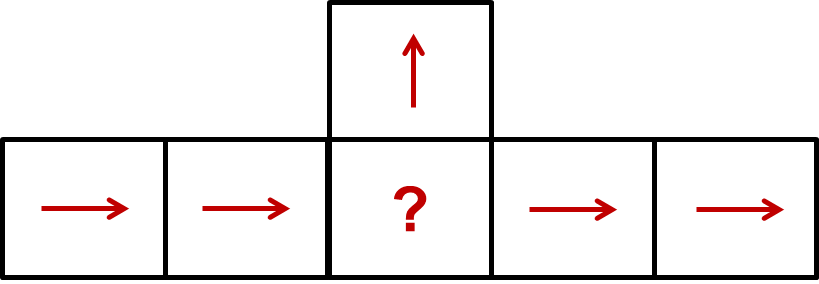
\includegraphics[scale=0.50]{BranchingProblem}
        \end{center}
    \end{frame}
    \begin{frame}{Staggered Spatial Grid}
        Mass and energy grid:\\
        \begin{center}
            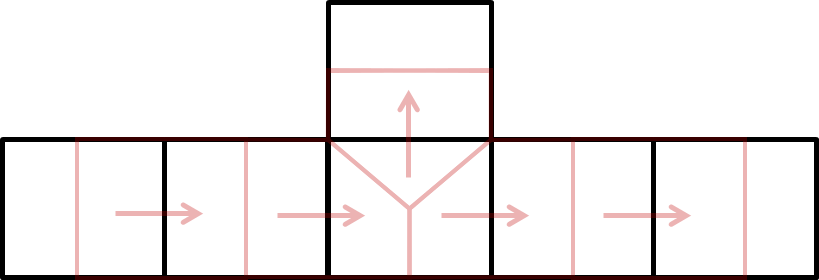
\includegraphics[scale=0.40]{Staggered_Control}
        \end{center}
        Momentum grid:\\
        \begin{center}
            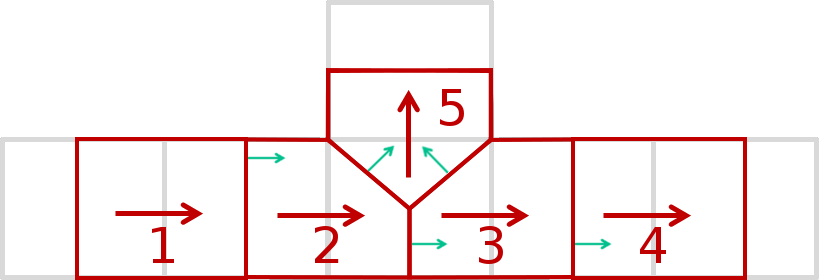
\includegraphics[scale=0.40]{Staggered_Momentum-NumberedWNormals}
        \end{center}
    \end{frame}
 

    \subsection*{Discretized Forms}
    \begin{frame}{Semi-Discretized Control Volume Equations}
        Mass and energy for control $k$:
        \begin{align}
            \deriv{}{t}\!\IntV \rho_k \dV  &= s^\rho_k V_k + \sum_{n=1}^{N} u_n \rho_{d,n} A_n \\[1em]
            \deriv{}{t}\! \IntV \rho i \dV &= s^e_k V_k + \sum_{n=1}^{N} u_n \rho{h}_{d,n} A_n
        \end{align}
    \end{frame}
    
    
    \begin{frame}{Semi-Discretized Momentum Cell Equation}
        Momentum for momentum cell $k$:
        \begin{equation}
            \deriv{}{t}\! \IntV \rho u_k \dV = 
                (\rho_k g_k + s^u_k)\,V_k 
                - \sum_{n=1}^{N}   (P_n z_n +  u_{\text{\textsc{i}},n} \rho{u}_{d,n}) A_n 
                - \frac{1}{2} f\subs{\textsc{d},k}\,\frac{L\subs{char,k}}{D\subs{eff,k}}\,\Abs(\rho{u}_k) u_k A_k
        \end{equation}
    \end{frame}
    
    
    
    \begin{frame}{Time Stepping}
        Semi-discrete equations are now of the form:
        \begin{equation}
            \pdt \qi = D_i(\qi)
        \end{equation}
        
        Various choices of stepping over a time step $p$:
        \begin{align}
            \qi^{p} - \qi^{p-1} &= \Delta{t}\,D_i(\qi^{p-1}) \\
            \qi^{p} - \qi^{p-1} &= \Delta{t}\,D_i(\qi^{p}) \\
            \qi^{p} - \qi^{p-1} &= \tfrac{1}{2}\Delta{t}\,\left[D_i(\qi^{p-1}) + D_i(\qi^{p})\right]
        \end{align}
    \end{frame}



% --------------------------------------------------- %
%                   Numerics: Solver                  %
% --------------------------------------------------- %
\section{JFNK}
    \begin{frame}{Full discretized equations}
        Consider the Implicit Euler full discretization:
        \begin{equation}
            \qi^{p} - \qi^{p-1} = \Delta{t}\,D_i(\qi^{p})
        \end{equation}
        
        How do you find $\qi^{p}$ to satisfy that equations assuming $D_i$ is nonlinear?
    \end{frame}
    
    \subsection*{Newton-Raphson}
    \begin{frame}{Newton-Raphson: Procedure}
        Put the equation into ``residual'' form
        \begin{equation}
            r(\qi^{p}) = \qi^{p} - \qi^{p-1} - \Delta{t}\,D_i(\qi^{p})
        \end{equation}
        and search for the vector $\qi^{p}$ that makes $r(\qi^{p})$ equal to $0$ (or close enough).
        \vfill
        Common search technique is Newton-Raphson method:
        \begin{align}
            \text{Solve } \partial_{\qi} r(\qi^{p})\,\Delta{\qi^{p}} &= -r(\qi^{p}) \\
            \qi^{p} &= \qi^{p} + \Delta{\qi^{p}}
        \end{align}
    \end{frame}
    \begin{frame}{Newton-Raphson: Problems}
        \begin{Itemize}
            \item{Calculating the Jacobian $\partial_{\qi} r(\qi^{p})$ can be time and memory intensive.}
            \item{Solving the linear system is likewise difficult}
        \end{Itemize}
    \end{frame}

    \subsection*{JFNK}
    \begin{frame}{JFNK}
        JFNK: Jacobian-Free Newton-Krylov method.
    \end{frame}
    \begin{frame}{Krylov method}
        A particular way of solving the linear system $A x = b$ :
        \begin{enumerate}
            \item{Compute a search direction $z_n$:
                \begin{equation}
                    z_n = \begin{cases}
                        r_{n-1} \quad \text{if } r_{n-1} < r_{n-2} \\
                        v_{n-1} \quad \text{otherwise}
                    \end{cases}
                \end{equation}
            }
            \item{Update a QR factorization:
                \begin{equation}
                    [A\,z_1,A\,z_2,...,A\,z_n] = V_n R_n
                \end{equation}
            }
            \item{Update residual:
                \begin{equation}
                    r_n = r_{n-1} - v_n^{\text{T}} r_{n-1}  v_n
                \end{equation}
            }
            \item{Solve the system
                \begin{equation}
                    R_n w_n = [v_1^{\text{T}} r_{1} ,...,v_n^{\text{T}} r_{n-1}]^{\text{T}};
                    \quad
                    x_n = x_0 + [z_1,...,z_n]w_n
                \end{equation}
            }
        \end{enumerate}
    \end{frame}
        
        
        \begin{frame}{Approximate Jacobian}
        Important part to notice
            \begin{equation}
                [A\,z_1,A\,z_2,...,A\,z_n]
            \end{equation}
        The only new computation every iteration is $A z_n$ (matrix-vector product).
        \vfill
        Jacobian-Free method uses the following finite difference relation:
        \begin{equation}
            \partial_{\qi} r(\qi^{p}) z_n \approx \frac{r(\qi^{p} + \varepsilon z_n) - r(\qi^{p})}{\varepsilon}
        \end{equation}
        \vfill
        Instead of creating the Jacobian, approximate its existence using this formula (Jacobian-free) in a Krylov Method.
        \end{frame}
        \begin{frame}{Jacobian-Free Newton-Krylov}
        \only<1>{
        A particular way of solving the linear system $A x = b$ :
        \begin{enumerate}
            \item{Compute a search direction $z_n$:
                \begin{equation}
                    z_n = \begin{cases}
                        r_{n-1} \quad \text{if } r_{n-1} < r_{n-2} \\
                        v_{n-1} \quad \text{otherwise}
                    \end{cases}
                \end{equation}
            }
            \item{Update a QR factorization:
                \begin{equation}
                    [A\,z_1,A\,z_2,...,A\,z_n] = V_n R_n
                \end{equation}
                \vskip0.92em
            }
            \item{Update residual:
                \begin{equation}
                    r_n = r_{n-1} - v_n^{\text{T}} r_{n-1}  v_n
                \end{equation}
            }
            \item{Solve the system
                \begin{equation}
                    R_n w_n = [v_1^{\text{T}} r_{1} ,...,v_n^{\text{T}} r_{n-1}]^{\text{T}};
                    \quad
                    x_n = x_0 + [z_1,...,z_n]w_n
                \end{equation}
            }
        \end{enumerate}
        }
        \only<2>{
        A particular way of solving the linear system $A x = b$ :
        \begin{enumerate}
            \item{Compute a search direction $z_n$:
                \begin{equation}
                    z_n = \begin{cases}
                        r_{n-1} \quad \text{if } r_{n-1} < r_{n-2} \\
                        v_{n-1} \quad \text{otherwise}
                    \end{cases}
                \end{equation}
            }
            \item{Update a QR factorization:
                \begin{equation}
                    [z_1, \frac{r(\qi^{p} + \varepsilon z_2) - r(\qi^{p})}{\varepsilon},...,\frac{r(\qi^{p} + \varepsilon z_n) - r(\qi^{p})}{\varepsilon}] = V_n R_n
                \end{equation}
            }
            \item{Update residual:
                \begin{equation}
                    r_n = r_{n-1} - v_n^{\text{T}} r_{n-1}  v_n
                \end{equation}
            }
            \item{Solve the system
                \begin{equation}
                    R_n w_n = [v_1^{\text{T}} r_{1} ,...,v_n^{\text{T}} r_{n-1}]^{\text{T}};
                    \quad
                    x_n = x_0 + [z_1,...,z_n]w_n
                \end{equation}
            }
        \end{enumerate}
        }
    \end{frame}





    % --------------------------------------------------- %
    %                     Stability: Intro                %
    % --------------------------------------------------- %
    \section{Stability}
    \subsection*{Derivation}
    \begin{frame}[label=Perturbation]{Perturbation equations}
        Assumed that the true solution is a summation of a steady-state and a transient
        \begin{equation}
            \q_i(x_i,t) = \qSS_i(x_i) + \dq_i(x_i,t).
        \end{equation}
        
        \onslide<2->{
            General nonlinear perturbation equation (\hyperlink{StabilityDiagrams}{diagrams}):
            \begin{equation}
                \pderiv{\dq_i}{t}  + \pderiv{}{x_j} \left[f_{ij}(\qSS_i + \dq_i)\right] = s_i(\qSS_i + \dq_i) 
                \label{Eqn:NonlinearStabilityEquation}
            \end{equation}
        }
        
        \onslide<3->{
            Taylor expansion about perturbation (neglecting H.O.T.) yields general linear perturbation equation:
            \begin{equation}
                \pderiv{\dq_i}{t}  + \pderiv{}{x_j} \left[\pderiv{f_{ij}}{\qSS_k{}}\dq_k\right] = \pderiv{s_i}{\qSS_k{}}\dq_k 
                \label{Eqn:GeneralLinearizedCLaw}
            \end{equation}
        }
    \end{frame}



    % --------------------------------------------------- %
    %                     Stability: Intro                %
    % --------------------------------------------------- %
    \subsection*{Linear Solutions}
    \begin{frame}{Solution method of general linear equations}
        Perturbations still part of spatially varying PDE.
        
        Discretizing like full transient equations will yield spurious, positive eigenvalues from mass/energy advection.
        
        Solution: integration over entire system and isolate global time-evolution on left-hand side:
        \begin{equation}
            \pdt\dq_i(t) = 
                \frac{1}{\int_\Omega \dV} \left[\int_\Omega\pderiv{s_i}{\qSS_k{}}\dV - 
                \int_\S\pderiv{f_{ij}}{\qSS_k{}}n_j\dS\right] \dq_k(t)
        \end{equation}
        
    \end{frame}
    \begin{frame}{Solution method of thermohydraulic system}
    
    \only<1>{
        Apply to mass, energy, momentum system:
        
        \begin{align}
            \deriv{}{t}
            \begin{bmatrix}
                \delta\mkern-2mu\rho \\ \delta\mkern-2mu\rho i \\ \delta\mkern-2mu\rho u_z 
            \end{bmatrix}
             &= 
            -\pdj
            \left(
                \begin{bmatrix}
                    \partial_{q_k}(\rho u_j)\\[1em]
                    \partial_{q_k}[(\rho{i} + P) u_j]\\[1em]
                    \partial_{q_k}(u_j \rho u_z + P \delta_{ij}z_i - \tau_{ij}z_i) 
                \end{bmatrix}
                \delta\mkern-2mu q_k
            \right)
            + 
            \left(
            \begin{bmatrix}
                \partial_{q_k} ( s^\rho )\\
                \partial_{q_k}(s^e )\\
                \partial_{q_k}(\rho g_z + s^u_z ) 
            \end{bmatrix}
                \delta\mkern-2mu q_k
            \right)
        \end{align}
    }
        
    \only<2->{
        Integrating to the skin of the system and eliminating terms that vanish:
        \begin{align}
            \deriv{}{t}
            \begin{bmatrix}
                \delta\mkern-2mu\rho \\ \delta\mkern-2mu\rho i \\ \delta\mkern-2mu\rho u_z 
            \end{bmatrix}
             &= 
            \frac{1}{V_{\text{sys}}}
            \begin{bmatrix}
                0 & 0 & 0 \\
                0 & 0 & 0 \\
                \alpha_\rho & \alpha_{\rho i} & \alpha_{\rho u_z} 
            \end{bmatrix}
            \begin{bmatrix}
                \delta\mkern-2mu\rho \\ \delta\mkern-2mu\rho i \\ \delta\mkern-2mu\rho u_z 
            \end{bmatrix},
        \end{align}
        where $\alpha_* = -\int_{\S}\partial_{*}\Delta{P}_{\text{dar}}\dS$
     }
    
    \only<3>{
        \vfill{}
        With the solution
        \begin{align}
    \begin{bmatrix}
        \delta\mkern-2mu\rho(t) \\ \delta\mkern-2mu\rho i(t) \\ \delta\mkern-2mu\rho u_z(t) 
    \end{bmatrix}
     &= 
    \begin{bmatrix}
        1 & 0 & 0 \\
        0 & 1 & 0 \\
        \frac{\alpha_\rho}{\alpha_{\rho u_z}}     \left(e^{\tilde{\alpha} t} - 1 \right) &
        \frac{\alpha_{\rho i}}{\alpha_{\rho u_z}} \left(e^{\tilde{\alpha} t} - 1 \right) &
        e^{\tilde{\alpha} t}
            \end{bmatrix}
            \begin{bmatrix}
                \delta\mkern-2mu\rho(0)\\ \delta\mkern-2mu\rho i(0) \\ \delta\mkern-2mu\rho u_z(0) 
            \end{bmatrix},
        \end{align}
            where $\tilde{\alpha} = \alpha_{\rho u_z} / V_{\text{sys}}$.
    }
    \end{frame}






    % --------------------------------------------------- %
    %                         Results                     %
    % --------------------------------------------------- %
    \section{Results}
    \begin{frame}{Methodology}
    \begin{enumerate}
        \item All closed-loop systems exhibit a singular steady-state solution.
        \item Solution: perform a transient calculation that provided diagonal regularity and run transient to a stationary-state using all previous equations and tools.
        \item Once the steady-state is attained, computer the eigenvalues and examine.
    \end{enumerate}
    \end{frame}
    \begin{frame}{Primary Test Loop}
        \begin{columns}
            \begin{column}[T]{0.45\textwidth}
                \begin{enumerate}
                    \item 14 control volume / momentum cells
                    \item 1.4 meters high, 0.4 meters wide (3.5 aspect ratio)
                    \item 0.1 meter hydraulic diameter
                \end{enumerate}
            \end{column}
            \hfill
            \begin{column}[T]{0.45\textwidth}
                \begin{figure}%
                    \centering
                    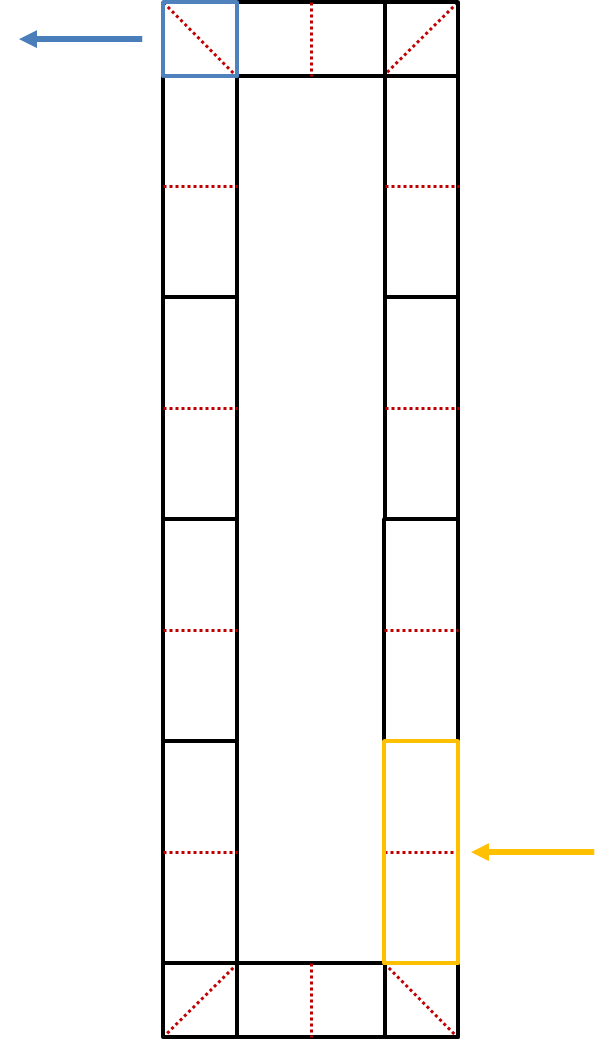
\includegraphics[scale=0.4]{TestLoop}%
                \end{figure}
            \end{column}
        \end{columns}
    \end{frame}
    
    
%??????????????????????????????????????????????????????????????????????
%??????????????????????????????????????????????????????????????????????
    \subsection*{Single Phase}
    \begin{frame}{Single Phase Results}
        
    \end{frame}
%??????????????????????????????????????????????????????????????????????
%??????????????????????????????????????????????????????????????????????    
    \subsection*{Two-Phase}
    \begin{frame}{Two-Phase Results}
        
    \end{frame}
%??????????????????????????????????????????????????????????????????????
%??????????????????????????????????????????????????????????????????????
%??????????????????????????????????????????????????????????????????????
%??????????????????????????????????????????????????????????????????????
    \subsection*{Two-Riser}
    \begin{frame}{Two-Riser Results}
        Two Riser Results?
    \end{frame}
%??????????????????????????????????????????????????????????????????????
%??????????????????????????????????????????????????????????????????????

    \subsection*{End}
    \begin{frame}[c]{Questions}
        \begin{center}
                ``The key to wisdom is this: constant and frequent questioning. 
                  For by doubting we are led to question, and by questioning we arrive at the truth.''\\
                \hfill --- Peter Abelard
        \end{center}
    \end{frame}







% ======================================================= %
%                       Appendix                          %
% ======================================================= %
\appendix
    
    
    \section{Supplements}
    
    
    % ====================================================================== %
    %                           Stagger/Collocated                           %
    % ====================================================================== %
    \subsection*{Staggered/Collocated}
    \begin{frame}[c,label=Meshes]{Staggered/Collocated}
        \begin{columns}
            \begin{column}[T]{0.4\textwidth}
                Staggered mesh:                
               \begin{center}
                   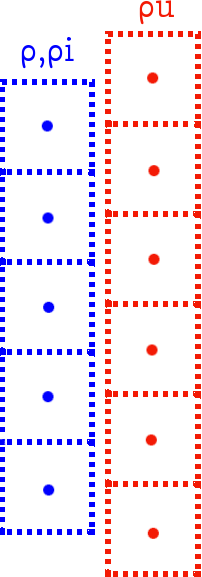
\includegraphics[height=2.2in]{StaggeredMesh}
               \end{center}
            \end{column}
            \hfill
            \begin{column}[T]{0.4\textwidth}
                Collocated mesh:
                \begin{center}
                    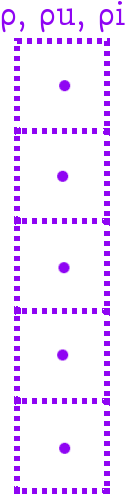
\includegraphics[height=2.2in]{CollocatedMesh}
                \end{center}
            \end{column}
        \end{columns}
    \end{frame}
    
    
    % ====================================================================== %
    %                      Rigorous/Non-rigorous                             %
    % ====================================================================== %
    \subsection*{Rigorous vs. Nonrigorous}
    \begin{frame}[c,label=Nonrigor]{Rigorous vs. Non-Rigorous}\label{Rigorous}
        \begin{columns}
            \begin{column}[T]{0.4\textwidth}
                Rigorous staggered mesh (CFD):                
               \begin{center}
                   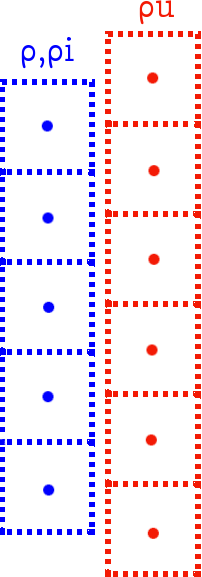
\includegraphics[height=2.2in]{StaggeredMesh}
               \end{center}
            \end{column}
            \hfill
            \begin{column}[T]{0.4\textwidth}
                Non-rigorous staggered mesh (System codes):
                \begin{center}
                    \null\vfill
                    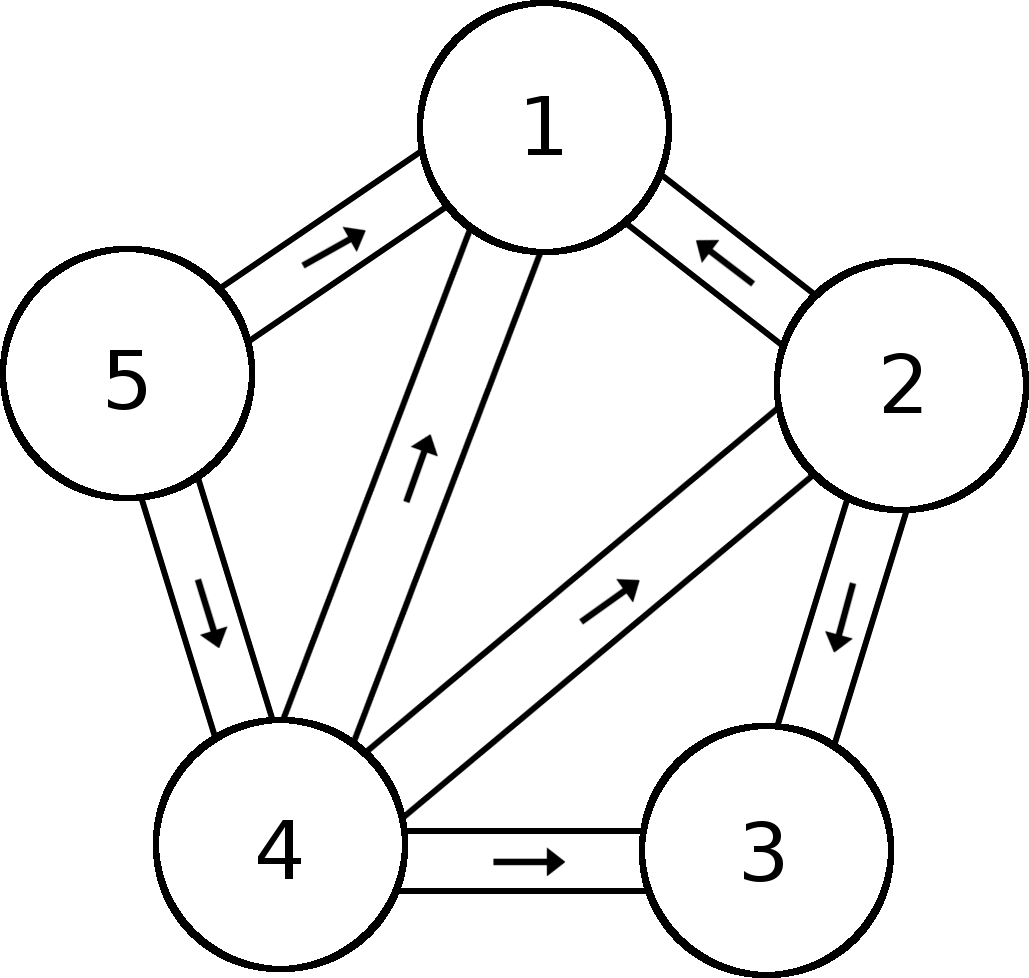
\includegraphics[scale=0.325]{NonrigorousMesh}
                    \null\vfill
                \end{center}
                \hfill\textit{\tiny\hyperlink{NonrigorMain}{return}}
            \end{column}
        \end{columns}
    \end{frame}
    
    
    % ====================================================================== %
    %                          Acoustic Speeds                               %
    % ====================================================================== %
    \subsection*{Acoustic Speeds}
    \begin{frame}[c,label=AcousticSpeeds]{Acoustic Speeds}
       \begin{center}
            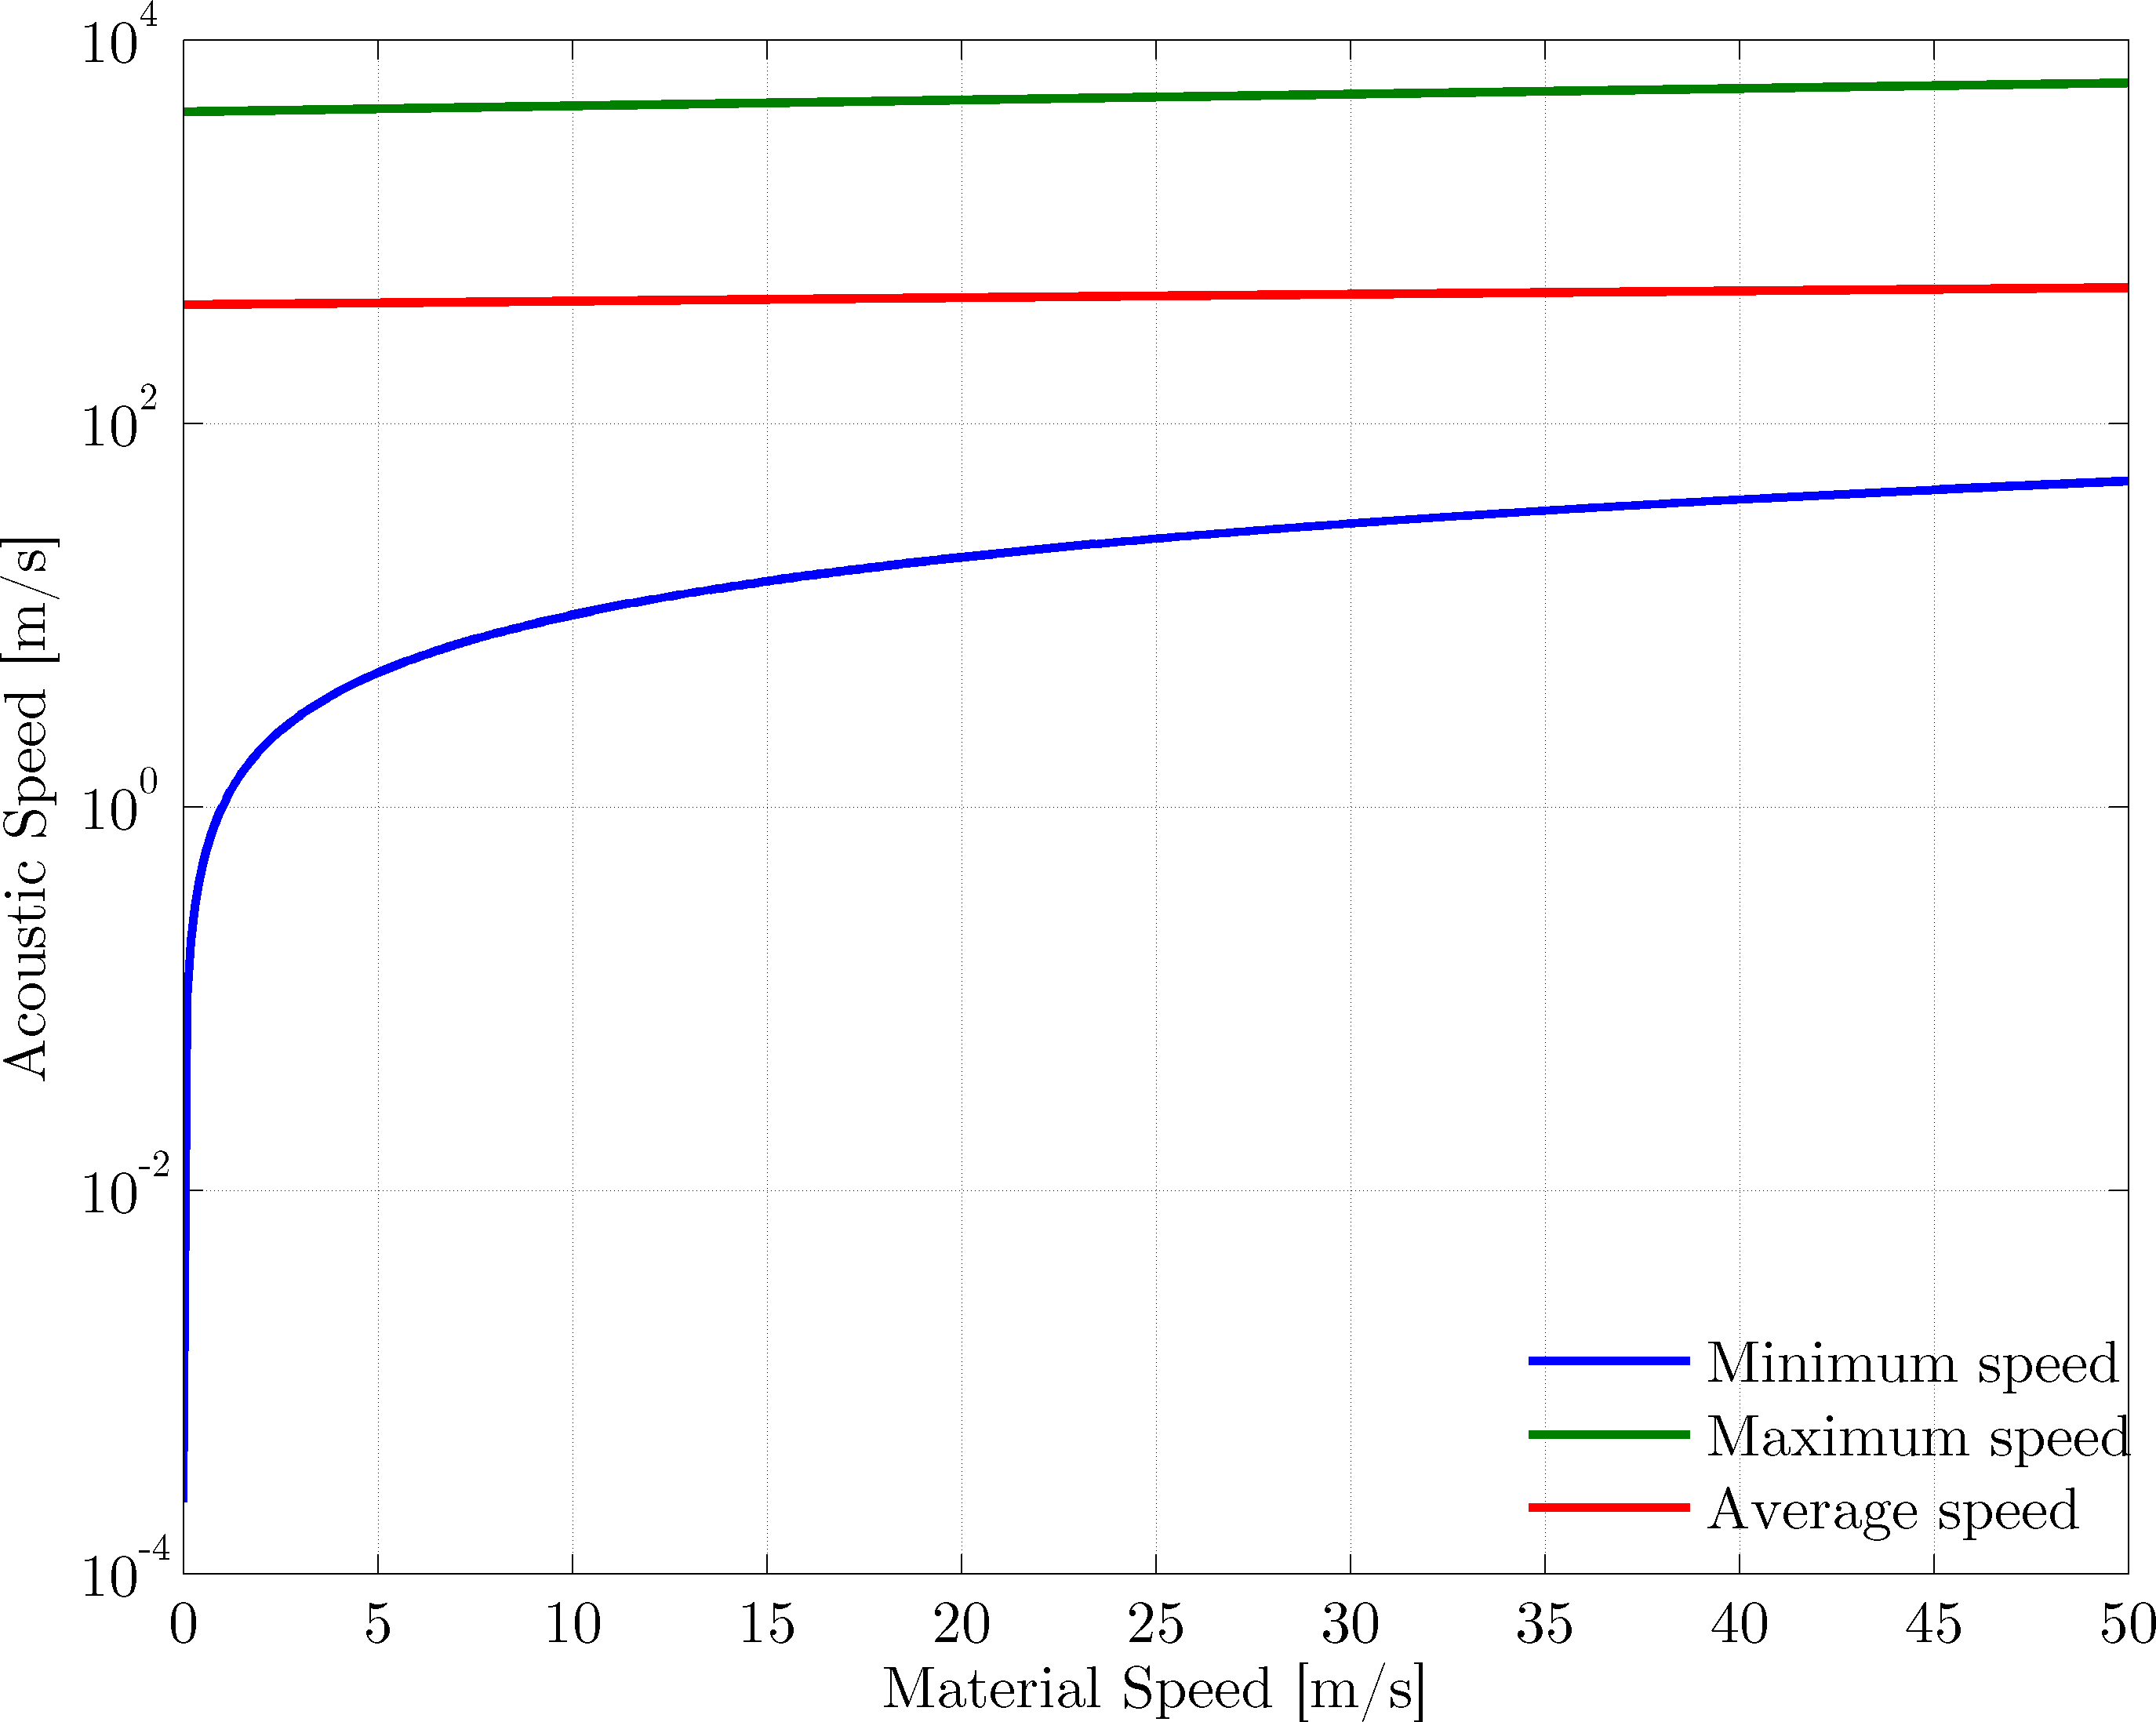
\includegraphics[height=2.2in]{AcousticSpeedVsMaterialSpeed}
       \end{center}
        \hfill\textit{\tiny\hyperlink{AcousticSpeedsMain}{return}}
    \end{frame}



    % ====================================================================== %
    %                          Non-simple, closed loop                       %
    % ====================================================================== %
    \subsection*{Non-simple, closed loop}
    \begin{frame}[c,label=NonsimpleClosedLoop]{Non-simple, closed loop}
        \begin{center}
            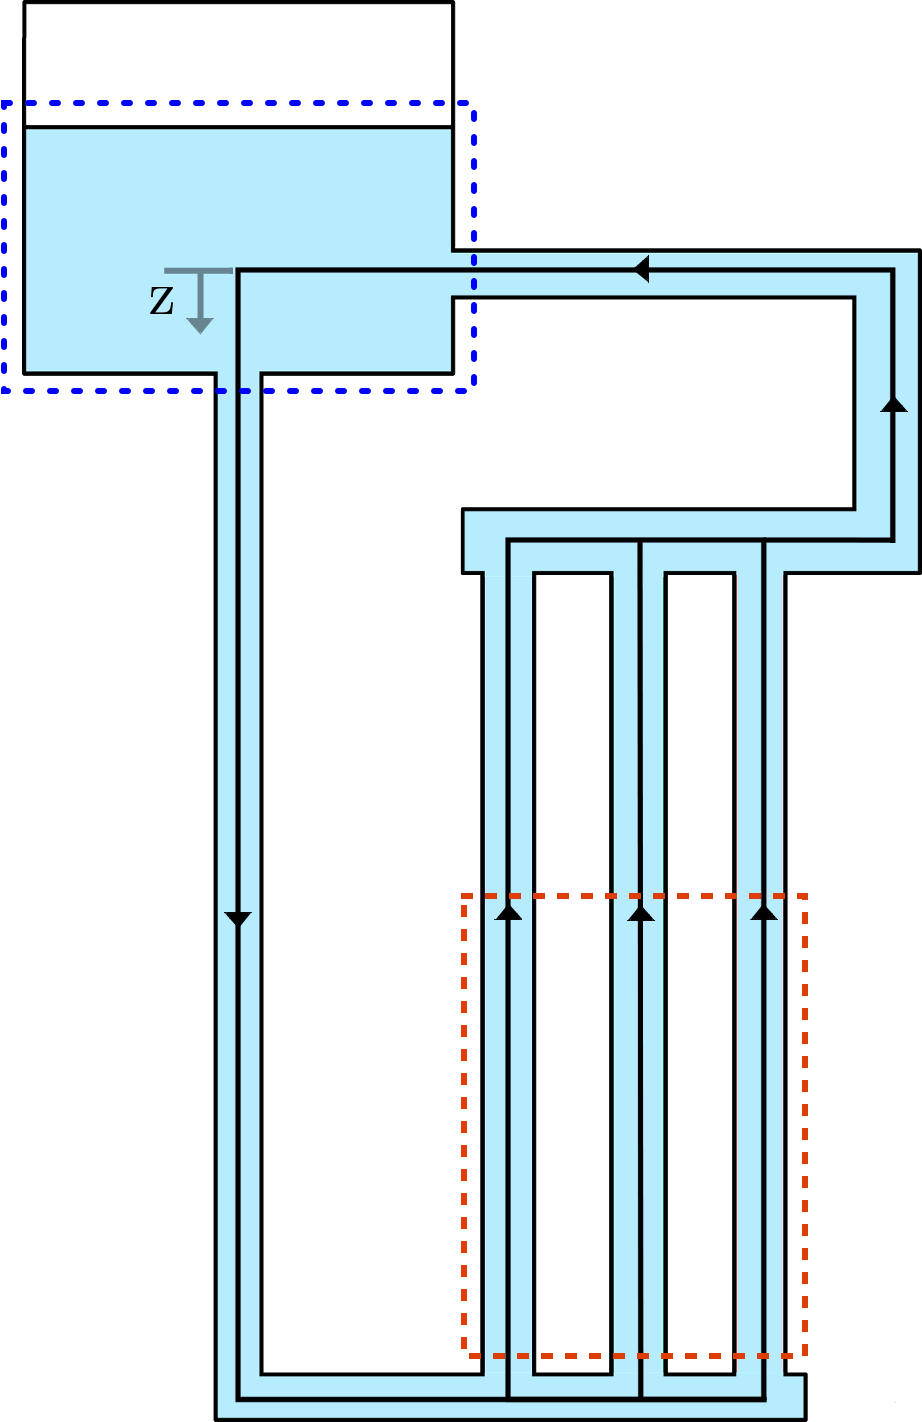
\includegraphics[height=2.2in]{ComputationalGeometry}
        \end{center}
    \end{frame}
    
    
    % ====================================================================== %
    %                          Non-simple, closed loop                       %
    % ====================================================================== %
    \subsection*{i-rho Space}
    \begin{frame}[c,label=irhoSpace]{$i$-\rho Diagram}
        \begin{center}
            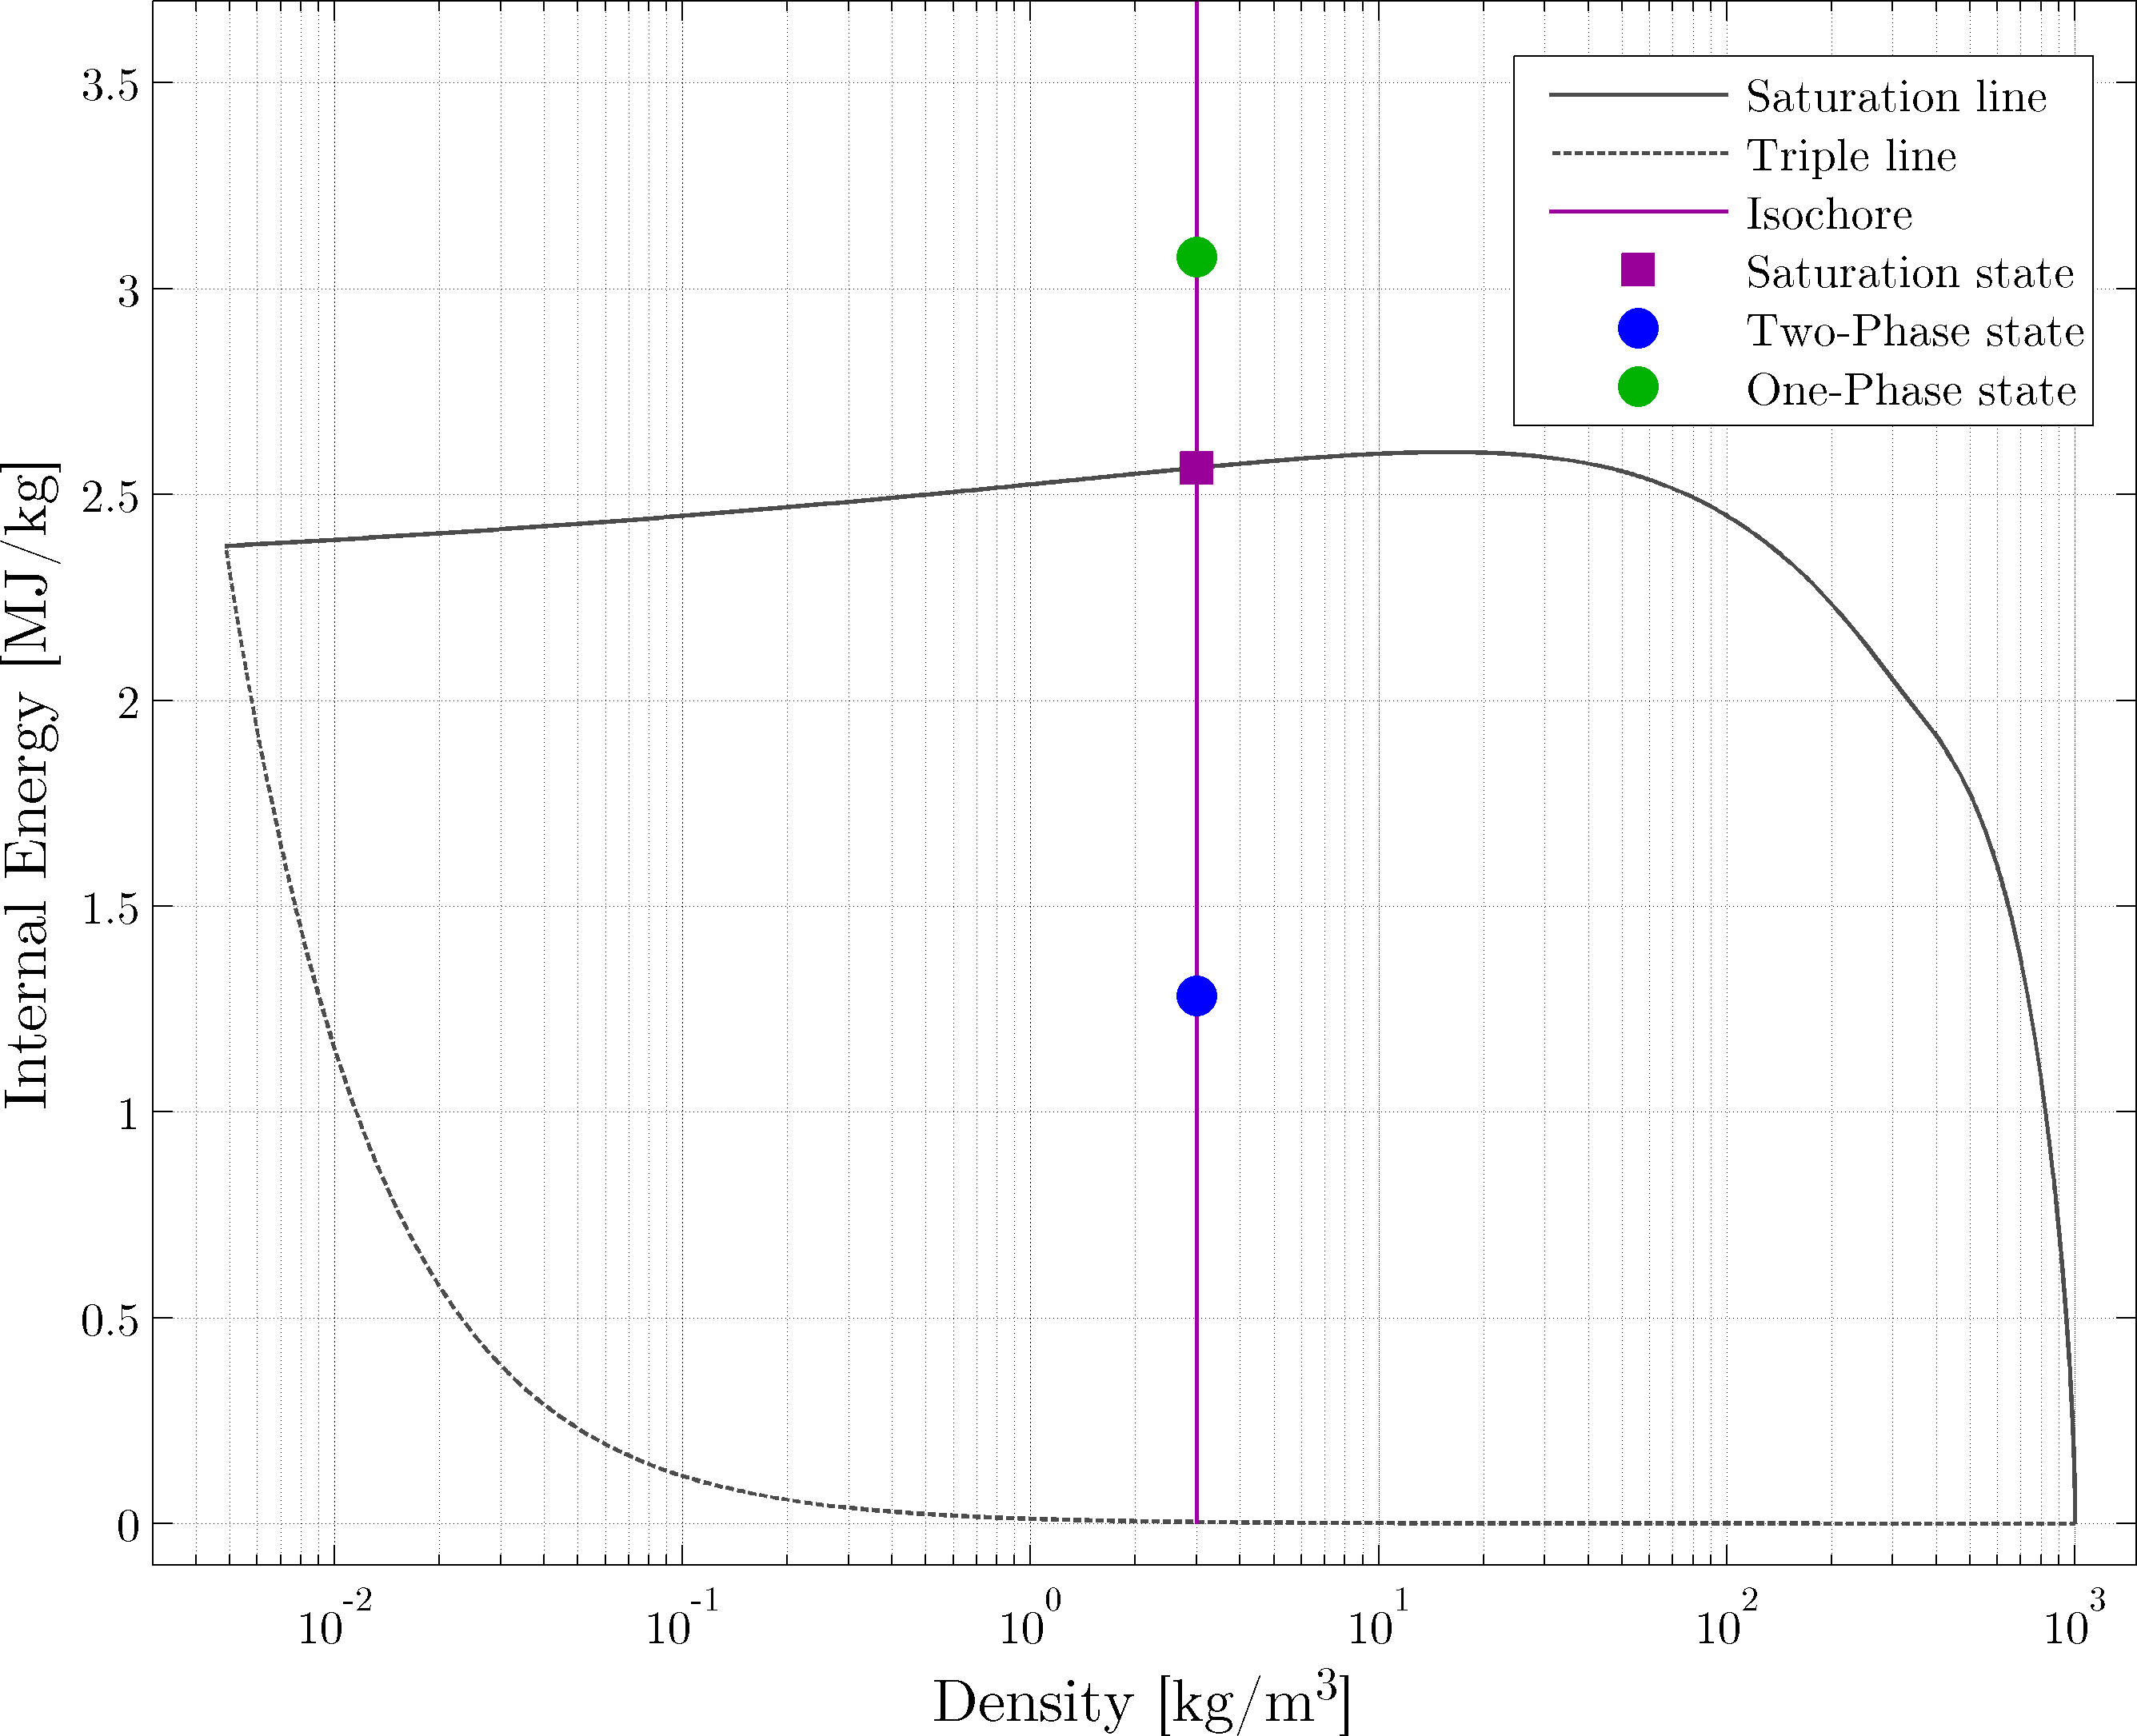
\includegraphics[height=2.2in]{InteEnergyVsDensity}
        \end{center}
        \hfill\textit{\tiny\hyperlink{EOS}{return}}
    \end{frame}
    
    
    
    % ====================================================================== %
    %                            Stability Diagrams                          %
    % ====================================================================== %
    \subsection*{Stability Diagrams}
    \begin{frame}[c,label=StabilityDiagrams]{Stability Diagrams}
        \begin{columns}
            \begin{column}[T]{0.4\textwidth}
                Linearly stable, nonlinearly unstable:
                \begin{center}
                    \vspace{0.09in}
                    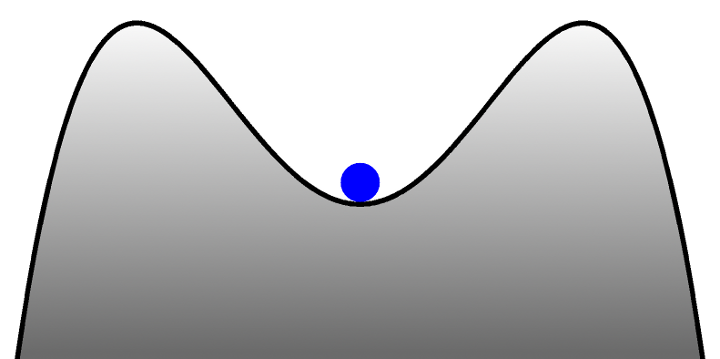
\includegraphics[height=0.91in]{LinearlyStableNonlinearlyUnstable}
                \end{center}
            \end{column}
            \hfill
            \begin{column}[T]{0.4\textwidth}
                Linearly unstable, nonlinearly stable:
                \begin{center}
                    \null\vfill
                    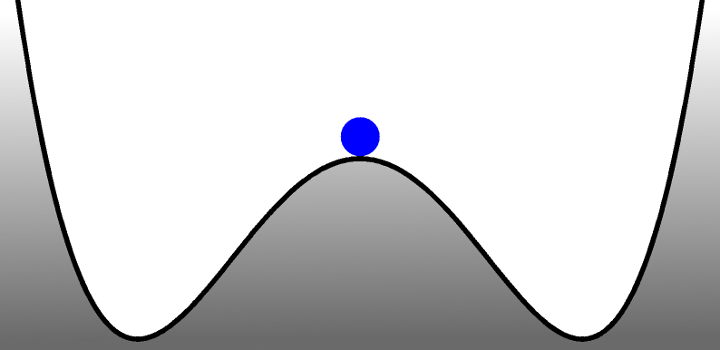
\includegraphics[height=0.83in]{LinearlyUnstableNonlinearlyStable}
                    \null\vfill
                \end{center}
                \hfill\textit{\tiny\hyperlink{Perturbation}{return}}
            \end{column}
        \end{columns}
    \end{frame} 
    
    
    
    % ====================================================================== %
    %                            Stability Diagrams                          %
    % ====================================================================== %
    \subsection*{System Mass flow: 4 days}
    \begin{frame}[c,label=MassFlow4Days]{System Mass flow: 4 days}
        \begin{center}
            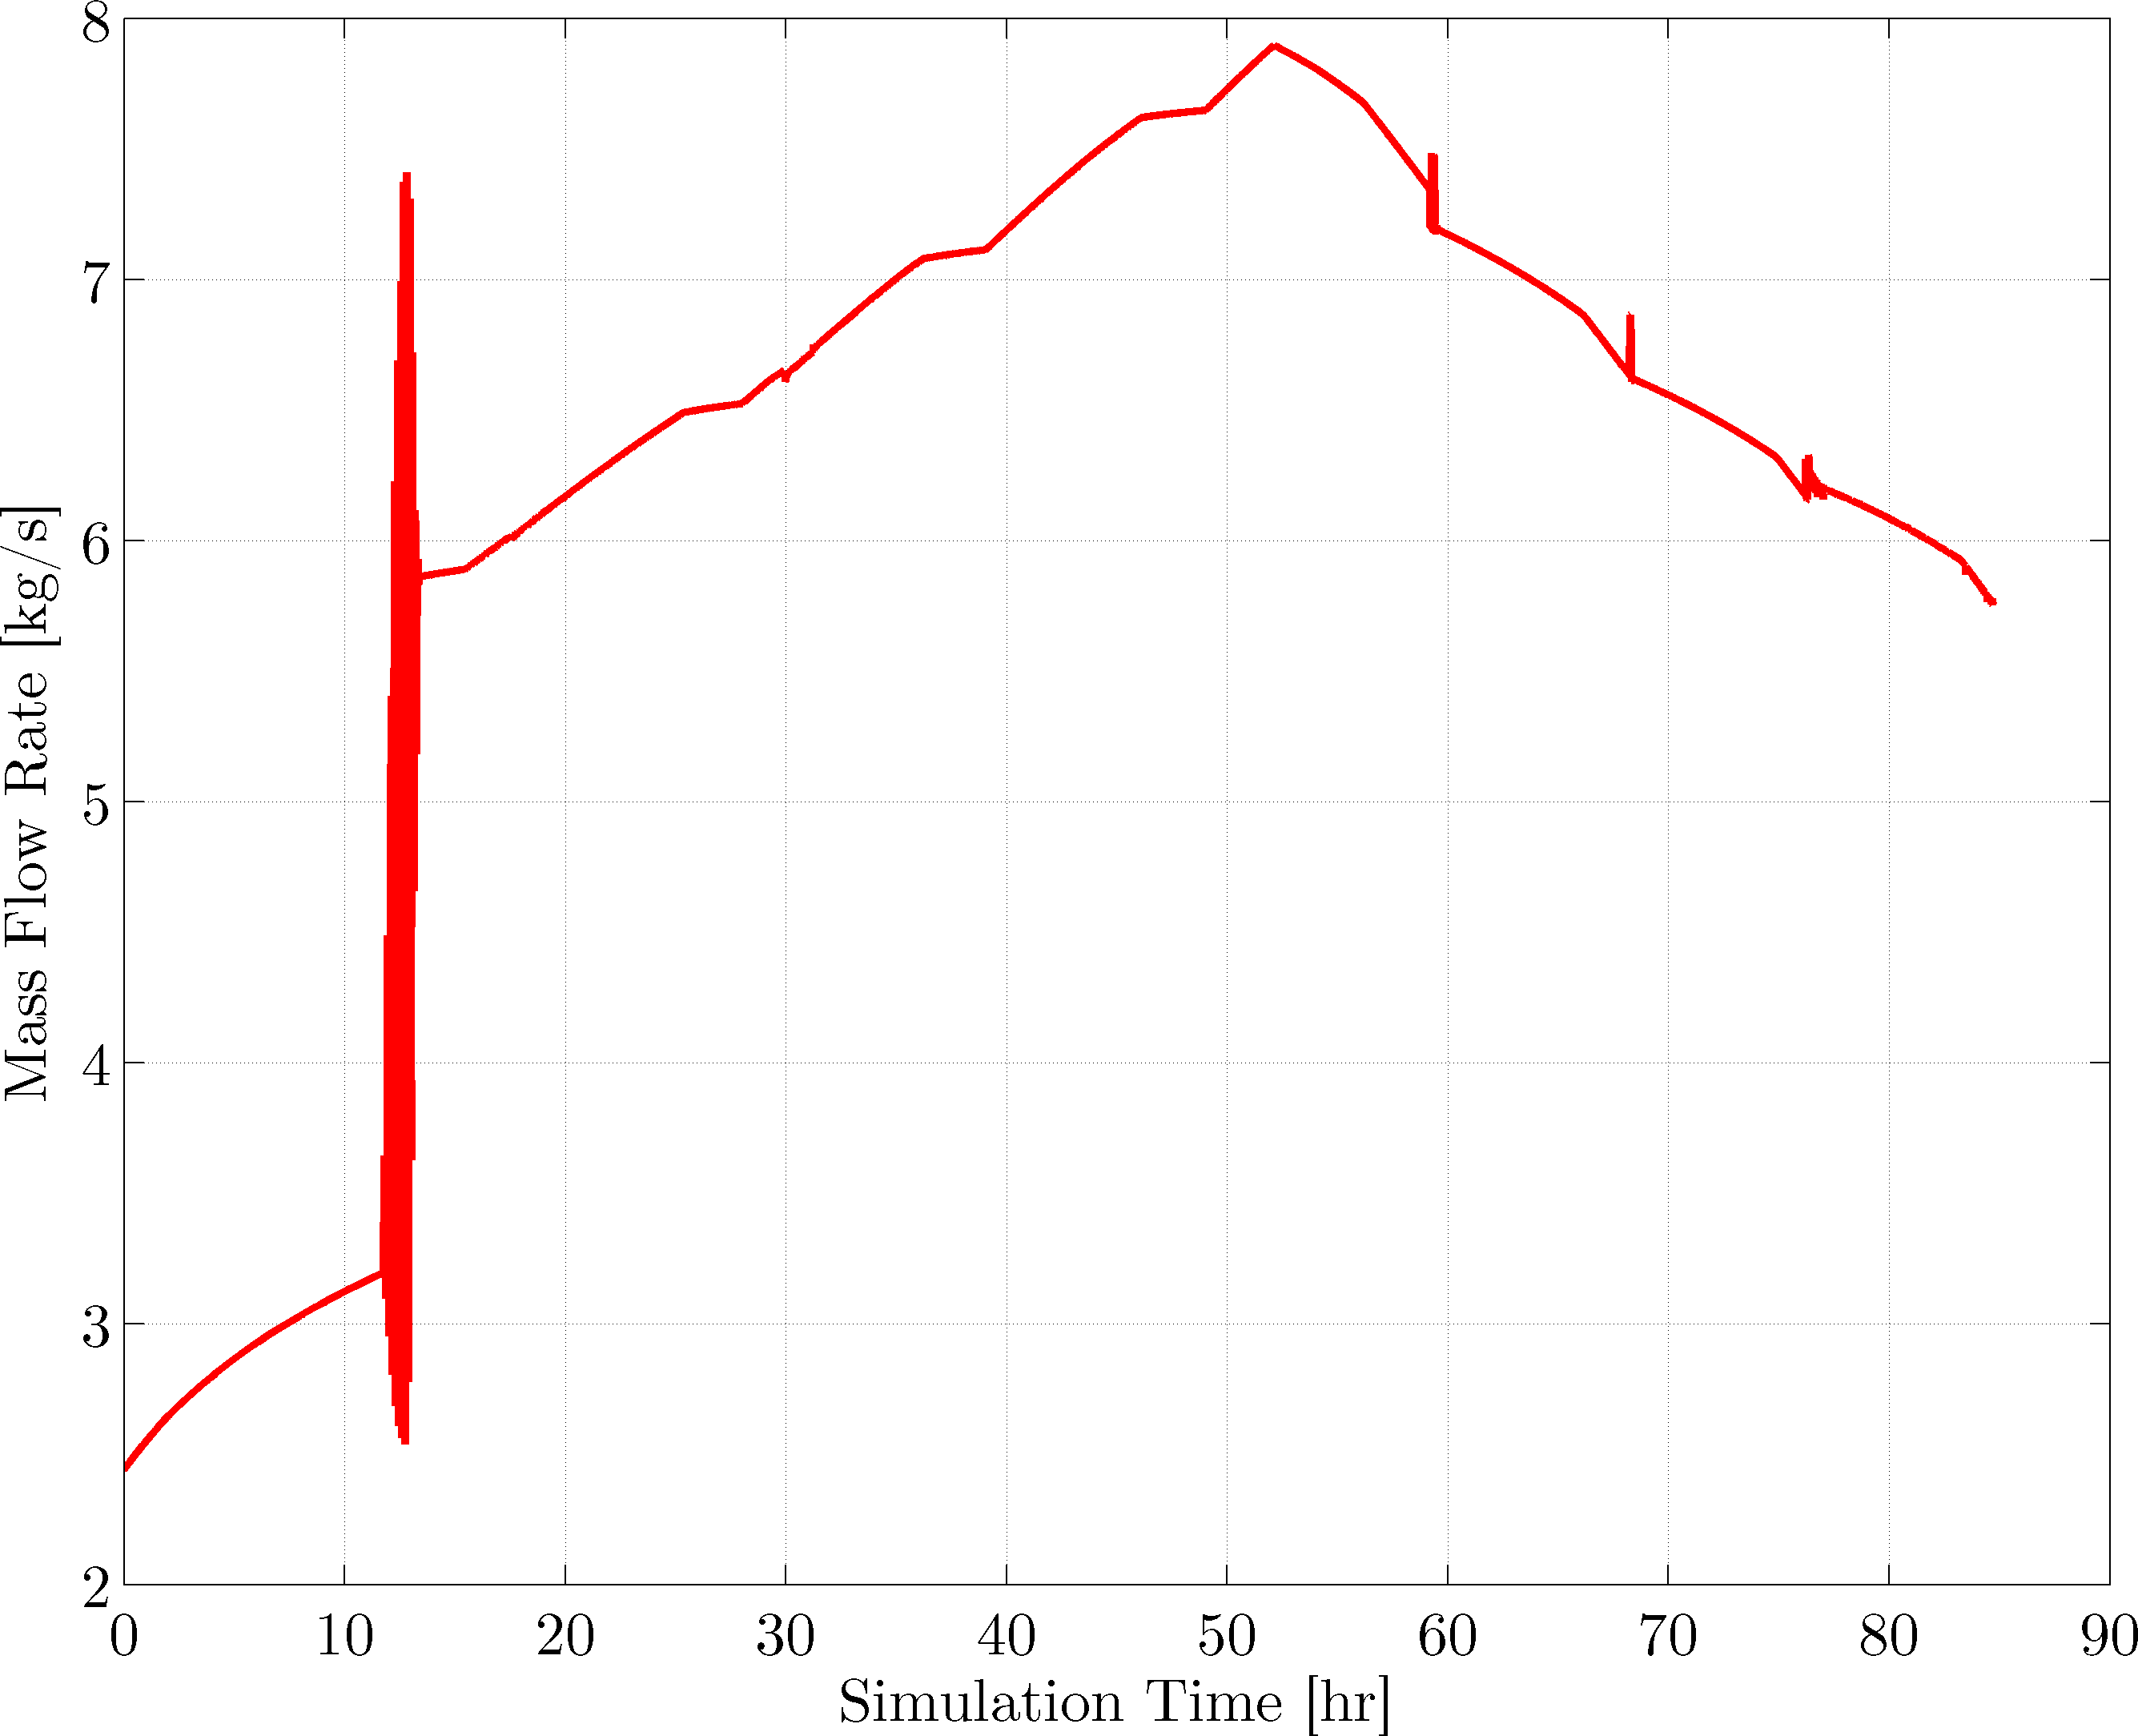
\includegraphics[height=2.4in]{MassRateFor4days}
        \end{center}
        \hfill\textit{\tiny\hyperlink{MassFlowAnnotate}{return}}
    \end{frame}
    
    
    
    % ====================================================================== %
    %                             Multiphase Model                           %
    % ====================================================================== %
    \subsection*{Multiphase Model}
    \begin{frame}[label=Multiphase]{Multiphase Model}
         \begin{equation}
            \renewcommand{\arraystretch}{2.2}
            \pdiff{}{t}\begin{bmatrix}
                           \rhok \\
                           \rhouk \\
                           \rhoik 
                        \end{bmatrix}
            + 
            \pdiff{}{z}\begin{bmatrix}
                            \rhouk                 \\
                            \uk\,    \rhouk  + P(\rho\subs{\phi},\ik)   \\
                            \uk\left[\rhoik  + P(\rho\subs{\phi},\ik)\right]
                        \end{bmatrix}
                     = 
        \end{equation}
        \begin{equation}\renewcommand{\arraystretch}{2.2}
            \begin{bmatrix}
                \mathbb{M}\subs{\phi} \\
                \rhok{g(z)} - \frac{\Keff\subs{,\phi}(\qCon)}{2} \uk\,|\rhouk| + \mathbb{P}\subs{\phi}  \\
                \dot{Q}\subs{add,\phi}(\qCon,z,t) + \mathbb{E}\subs{\phi}
            \end{bmatrix}
            \notag
        \end{equation}
    \end{frame}


\end{document}

